\chapter{Analysis techniques}

\intro{This chapter introduces the necessary toolset to perform the analyses within this thesis.}

\section{Event generation}

\myfigure{\label{fig:technique-mcevent} blb b sf sdfsdgs gfs dfg sfdgs dfsd fs dfs gfsdf gs dfs dgsgdfgds ssdsg fsdf asdf sdg sfgf gfgsfgs dfaf df szdg sg fgs fg sfgs df gds fsf sdgdfgfdgsd s df sdfds.}{
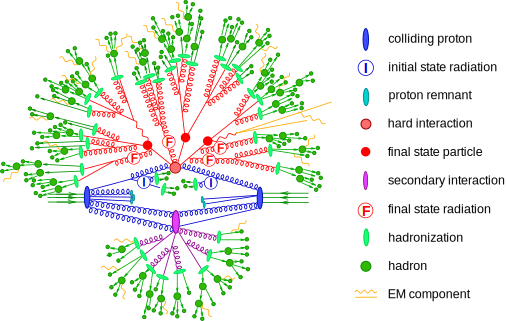
\includegraphics[scale=0.75]{figures/technique/shower.pdf}
}

matrix elements, integration, loops, shower simulation, matching schemes

\subsection{MadGraph and aMC{@}NLO}

\subsection{Powheg}

\subsection{Comphep}

\subsection{Pythia}

lund-string model

\subsection{Herwig}

\section{Top quark reconstruction}

neutrino solution, matching performance

\section{Boosted Decision Trees}
\cite{Hocker:2007ht}


\section{Template-based fitting}

likelihood, barlow-beeston method

\section{Fiducial objects}

dressed leptons, jet clustering, b-tagging

\section{Unfolding}

problems, regularization scheme, correlations, subway plot, alternative FBU
